\documentclass[12pt,a4paper]{article}
\usepackage[utf8]{inputenc}
\usepackage[T1]{fontenc}
\usepackage[provide=*,french]{babel}
\usepackage{graphicx}
\usepackage{geometry}
\usepackage{hyperref}
\usepackage[all]{hypcap}

\geometry{margin=2.5cm}

\begin{document}

% Page de garde
\begin{titlepage}
    \begin{center}
        \vspace*{2cm}
        {\huge\bfseries Devoir 3\par}
        {INFO4305\par}
        \vspace{2cm}
        {\Large Alec Jones\par}
        {\large A00216262\par}
        \vfill
    \end{center}
\end{titlepage}

\tableofcontents
\newpage

% Introduction
\section{Introduction}

% Objectif
\section{Objectif du TP}
 [Les objectifs du TP]

% Corps du rapport
\newpage
\section{Déroulement du TP}
\subsection{Partie 1}
Premièrement on doit d'abord installer Gpg4win, j'ai installer le logiciel à
l'aide du manager de paquets WinGet (voir la figure \ref{gpg4win}).

\begin{figure}[h]
    \centering
    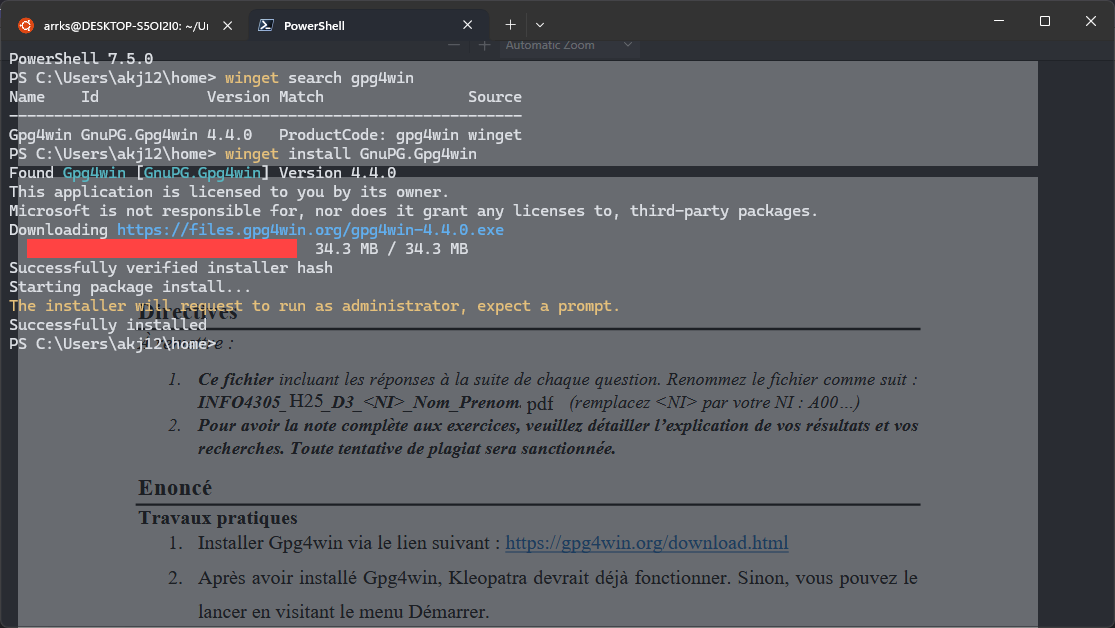
\includegraphics[width=0.8\textwidth]{../img/gpg4win.png}
    \caption{Installation de Gpg4win}
    \label{gpg4win}
\end{figure}

\subsection{Partie 2}
\subsubsection{Partie a}
Pour créer une paire de clé à l'aide de l'interface graphique, on doit ouvirir le logiciel
Kleopatra, ensuite on selectionne l'option new key pair (voir la figure \ref{kleopatra}).

\begin{figure}[h]
    \centering
    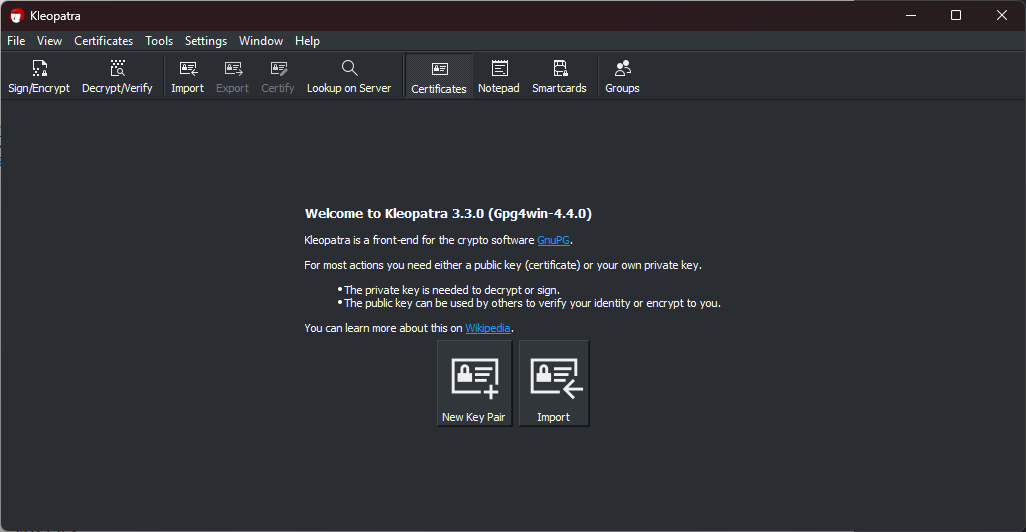
\includegraphics[width=0.8\textwidth]{../img/kleopatra.png}
    \caption{Menu initial Kleopatra}
    \label{kleopatra}
\end{figure}

Ensuite, on doit sélectionné options avancés et puis rsa2048.
On doit aussi remplir notre nom et notre courriel pour le certificat (voir \ref{newKey}).

\begin{figure}[ht]
    \centering
    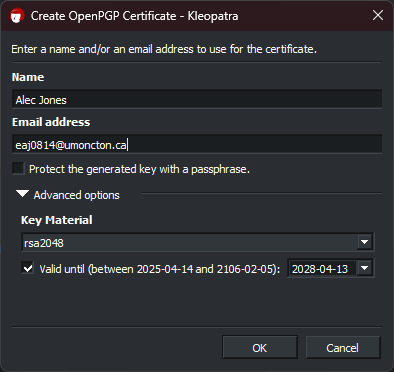
\includegraphics[width=0.8\textwidth]{../img/newKey.png}
    \caption{Création de clés dans Kleopatra}
    \label{newKey}
\end{figure}

\subsubsection{Partie b}
Pour créer une paire de clé en ligne de commande, vous pouvez utiliser la commande suivante dans un terminal :

\begin{verbatim}
gpg --full-generate-key
\end{verbatim}

Cette commande lance un assistant interactif vous permettant de choisir le type de clé, la longueur (par exemple, rsa2048 ou rsa4096)
et de renseigner les informations nécessaires (nom, adresse électronique, etc.). Une fois terminé, votre paire de clés sera générée et stockée dans votre trousseau GPG (voir figure \ref{newKey_cli}).

\begin{figure}[ht]
    \centering
    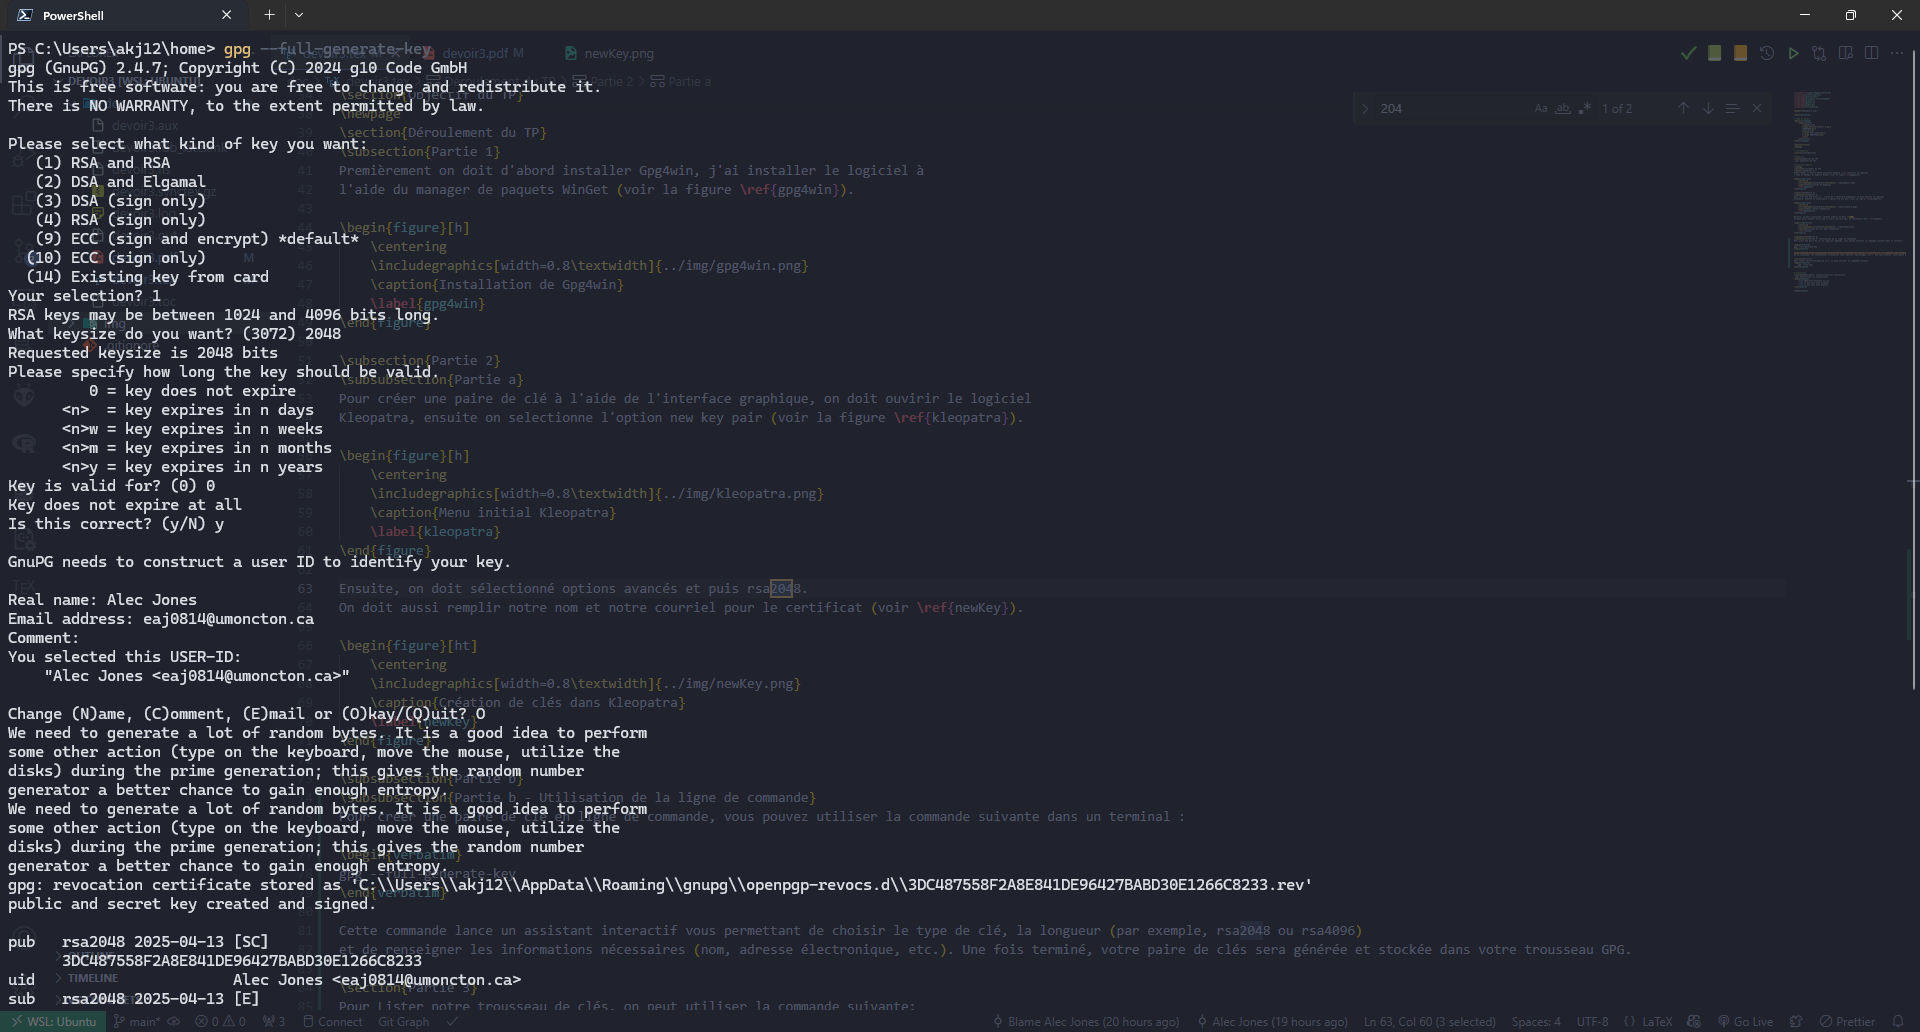
\includegraphics[width=0.8\textwidth]{../img/newKey_cli.png}
    \caption{Création de clés à l'aide de la ligne de commande}
    \label{newKey_cli}
\end{figure}

\subsection{Partie 3}
Pour Lister notre trousseau de clés, on peut utiliser la commande suivante:
\begin{verbatim}
    gpg --list-keys
\end{verbatim}
En exécutant la commande on appercois les deux clés créers précédément (voir figure \ref{listKeys}).

\begin{figure}[ht]
    \centering
    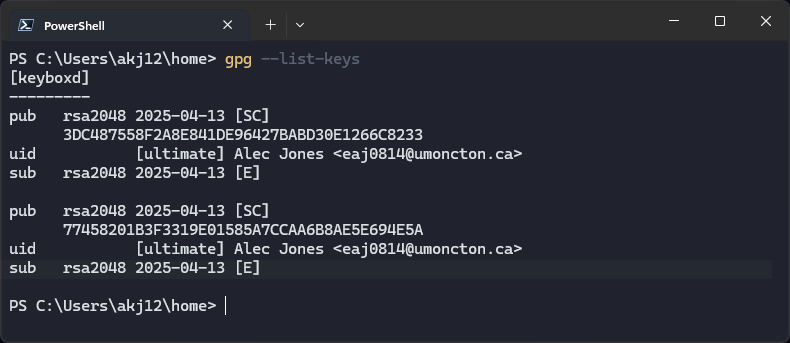
\includegraphics[width=0.8\textwidth]{../img/listKeys.png}
    \caption{Liste des clés}
    \label{listKeys}
\end{figure}

\subsection{Partie 4}
Pour exporter les clés publiques, on utilise la commande:
\begin{verbatim}
    gpg --armor --output maclé.asc --export UserID
\end{verbatim}
Puisqu'on spécifie le UserID, par example eaj0814@umoncton.ca,
qui à été utiliser dans les deux clés, on obtient la concaténation des deux dans un fichier.
On remarque alors que maclé.asc est éffectivement la concaténation des deux clés publiques créer tout à l'heure.

\subsection{Partie 5}
Pour chiffrer un fichier, on utilise la commande suivante (voir figure \ref{chiffre} pour un example):
\begin{verbatim}
    gpg -er UserID document.txt
\end{verbatim}

\begin{figure}[ht]
    \centering
    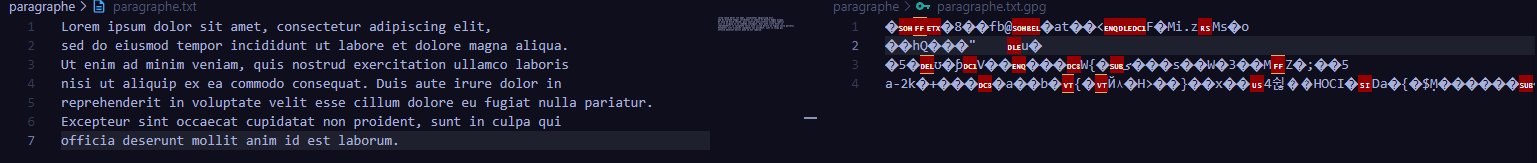
\includegraphics[width=0.8\textwidth]{../img/chiffre.png}
    \caption{text clair à gauche, chiffrer à droite}
    \label{chiffre}
\end{figure}

\subsection{Partie 6}
Si on voulais ensuite déchiffrer ce texte, on utiliserais la commande suivant :
\begin{verbatim}
    gpg --output doc --decrypt doc.gpg
\end{verbatim}

\subsection{Partie 7}
Pour signer un document et laisser le text en clair, on utilise la commande suivante (Voir la figure \ref{sign} pour example de résultat):
\begin{verbatim}
    gpg --clearsign document.txt
\end{verbatim}

\begin{figure}[ht]
    \centering
    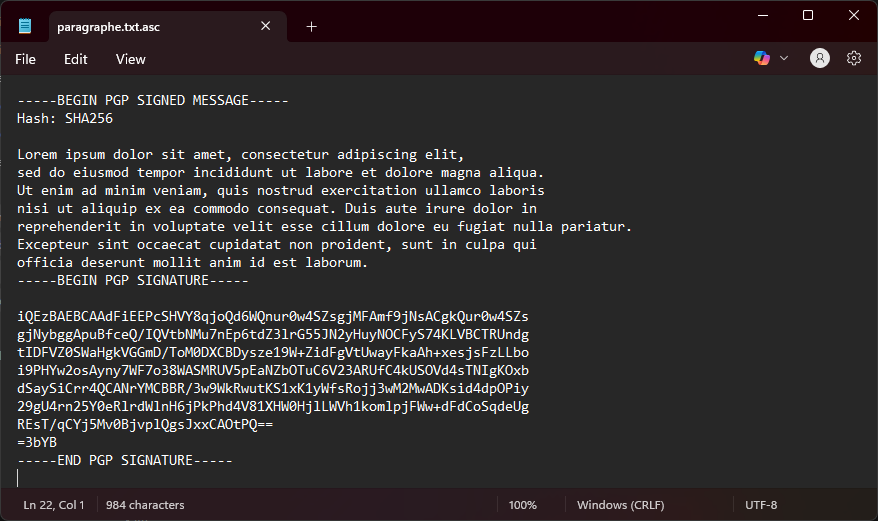
\includegraphics[width=0.8\textwidth]{../img/sign.png}
    \caption{Document signé}
    \label{sign}
\end{figure}

\subsection{Partie 8}
Pour vérifier la signature, on utilise la commande suivante (voir figure \ref{verif}):
\begin{verbatim}
    gpg --verify document.txt.asc
\end{verbatim}

\begin{figure}[ht]
    \centering
    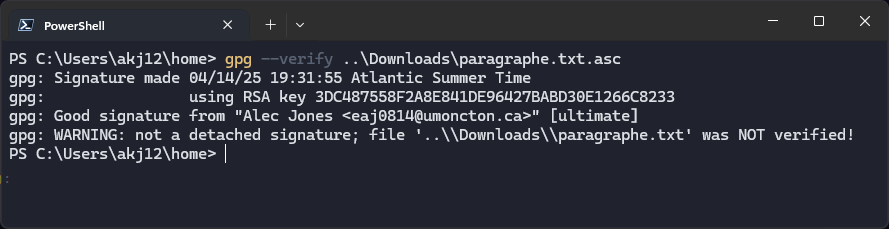
\includegraphics[width=0.8\textwidth]{../img/verif.png}
    \caption{Vérification de la signature}
    \label{verif}
\end{figure}

\subsection{Partie 9}
L'utilité de la signature dans ce contexte est de garantir l'intégrité du document et d'assurer que le document n'a pas été modifié depuis sa signature.
En vérifiant la signature, on peut s'assurer que le document provient bien de la personne qui l'a signé et qu'il n'a pas été altéré.
(voir figure \ref{verif_modif} pour un example de document modifier).

\begin{figure}[ht]
    \centering
    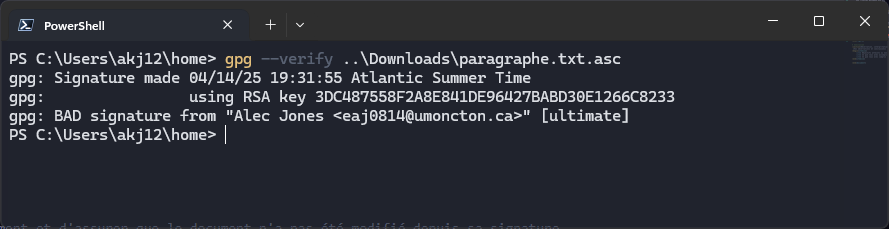
\includegraphics[width=0.8\textwidth]{../img/verif_modif.png}
    \caption{Vérification de la signature sur un document modifié, le premier mot a été enlevé}
    \label{verif_modif}
\end{figure}


% Conclusion
\section{Observation, interprétation et conclusion}
 [Vos observations et conclusions]
\begin{itemize}
    \item Objectifs atteints ou non
    \item Ce que vous avez accompli
    \item Ce que vous avez compris
\end{itemize}

\end{document}
